\section{Experience}

\subsection{Re-use of data from clinical information systems}

The UK National Institute of Health Research (NIHR) is funding an
\pounds 11m programme of work across five large university-hospital
partnerships: at Oxford, Cambridge, Imperial College London,
University College London, and Guy's and St.~Thomas'.  The aim of the
programme is to create the infrastructure needed to support data
re-use and translational research across these five institutions.

The programme, the NIHR Health Informatics Collaborative (HIC), was
initiated in 2013, with a focus upon five therapeutic areas: acute
coronary syndromes, renal transplantation, ovarian cancer, hepatitis,
and intensive care.  The scope was increased in 2015 to include other
cancers---breast, colorectal, lung, and prostate---and other
infectious diseases, including tuberculosis.

The key component of the infrastructure consists in repositories of
patient data within each of the five institutions.  The intention is
that these repositories should hold a core set of data for each
therapeutic area, populated automatically from clinical systems,
together with detailed documentation on the provenance and
interpretation of each data point.  

Researchers can use the documentation to determine the availability
and suitability of data for a particular study.  They can use it also
to determine comparability across institutions: whether there are any
local differences in processes or equipment that would have a bearing
upon the combination and re-use of the corresponding data.  Once a
study is approved, the repositories act as a single source of data,
avoiding the need for data flows from individual clinical systems.

The development of the infrastructure required the development of a
`candidate data set' for each therapeutic area, as a core list of data
points collected in the course of routine care that would have value
also in translational research.  Each institution then set out to
determine which information systems, within their organisation, could
be used to populate each of the candidate data sets: this was termed
the `data exploration exercise'.

The results of the exercise informed further development of the data
sets, and data flows were established.  To demonstrate and evaluate
the new capability, `exemplar research studies' were initiated in each
therapeutic area, using data from all five institutions.  

Each institution had a different combination of existing systems, a
different approach to data integration, and a different strategy for
informatics development.  It was not feasible or appropriate to
develop a common `data repository' product for installation.  Instead,
a set of data models were distributed, and each institution worked to
implement these using their own messaging, business intelligence, or
data warehousing technologies. 

None of the institutions had the capability to provide documentation
on the provenance and interpretation of their data in any standard,
computable format; the model or metadata aspect of the infrastructure
was entirely new.  It was this that drove---and continues to
drive---the development of a comprehensive model catalogue
application. 

At the start of the project, teams of clinical researchers and leading
scientists were given the responsibility of creating the candidate
data sets for each therapeutic area.  They did this by exchanging
spreadsheets of data definitions in email.  This proved to be a slow
process, and face to face meetings were needed before any real
progress could be made.

It proved difficult to properly represent repeating sections of the
dataset---corresponding to investigations or interventions that may
happen more than once for the same patient.  Researchers resorted to
Visio diagrams to try to explain how observations fitted into clinical
pathways or workflows---and discovered that there were significant
differences between pathways for the same disease at different
institutions.  

In one therapeutic area, these differences had a profound effect upon
the interpretation of certain observations, and the candidate dataset
was extended to include additional information on the pathway.  Due to
the complexity of the pathways involved, this was a time-consuming and
error-prone process.  Furthermore, the spreadsheets quickly became
inconsistent with the Visio diagrams.

The candidate datasets were distributed to the informatics teams at
the five institutions in the form of XML schemas.  At first, these
were created from scratch, rather than being generated.  There were
many requests for changes to the schemas; these proved difficult to
track and coordinate.

The exploration exercise itself was reported by adding columns to the
distributed versions of the candidate dataset spreadsheets, listing
the information systems containing the data points in question, or
suggested alternatives where there were significant differences due to
local systems and processes.

This was despite the availability of an initial version of the model
catalogue.  Researchers and local informatics teams preferred to work
with spreadsheets, having little or no knowledge of modelling
languages such as UML and no automatic support for model creation and
maintenance.  It fell to the software engineering team at the
coordinating centre to record the datasets and variations in the
catalogue.

While it was disappointing to have the researchers still working in
spreadsheets, the ability to generate XML schemas from models, and to
manage relationships between data items in different models and
different versions, proved invaluable.  In the second phase of the
project, with more therapeutic areas being added, researchers are
starting to abandon the spreadsheet mode of working, and are instead
maintaining the datasets as data models, in the catalogue.

\subsection{Coordination of clinical data acquisition}

The UK Department of Health, through the NIHR and the National Health
Service (NHS), is providing funding for the collection for the whole
genome sequencing of blood and tissue samples from patients with
cancer, rare disorders, and infectious disease.  A network of regional
Genomic Medicine Centres (GMCs) is being established to collect
samples and data, and to provide access to genomic medicine across the
whole of the country.

The results of the whole genome sequencing will be linked to detailed
information on each participant: clinical and laboratory information
drawn from health records, ontological statements regarding abnormal
features or conditions, and additional information obtained from the
participant or their representatives.  The information required will
depend upon the nature of the disease that the patient is suffering
from.  For example, information on breast density is required in the
case of breast cancer, but not for other diseases.

131 different diseases have been included in the sequencing programme
thus far.  Each disease corresponds to a different combination of
clinical and laboratory data points, a different set of ontological
statements, and a different set of questions for the participant.






Whilst that process was being carried out, some of these datasets were
added to the Model Catalogue, and the subject matter experts were
given visibility of the datasets already stored in the Model
Catalogue. At this point the Model Catalogue was already loaded with
datasets derived from the NHS Data dictionary such as COSD and from
the results of the NHIC work. Use of the toolkit resulted in the users
being able to very quickly assemble a new dataset from an existing
dataset; they were then able to go through each data element in turn
and compare it to an existing data element in another datamodel, a
process that is illustrated in Figure~\ref{fig:dataClassComparison}.

For the Genomics England exercise, the Models Catalogue has had a
social networking feature added, allowing messaging forums to be
automatically generated around a \emph{datamodel} or
\emph{dataclass}. This allows users to develop a new draft datamodel,
and then

From looking at the datasets we can see that in the first 2 major
datamodels produced X\% of data elements and dataclasses were derived
from existing sources, a fact entirely due to the use of the Model
Catalogue in the data curation process. Time to assemble a new
datamodel has been cut from months to weeks as a result of having a
single shared source for the datamodel, and having the means to
electronically comment on and discuss datamodel development in real
time as it is happening.

\begin{itemize}
	\item Data Elements can be used across different DataModels - favourites or shopping cart.
	\item Unique Identification of DataElements 
	\item Documentation can be automatically generated for review purposes
	\item Consistency checking carried out on data elements
	\item Generation of XSDs, XML, and Forms as output, interfacing with OpenClinica.
	\item Data Provenance
\end{itemize}
\lipsum[1-2]
\begin{figure*}  
	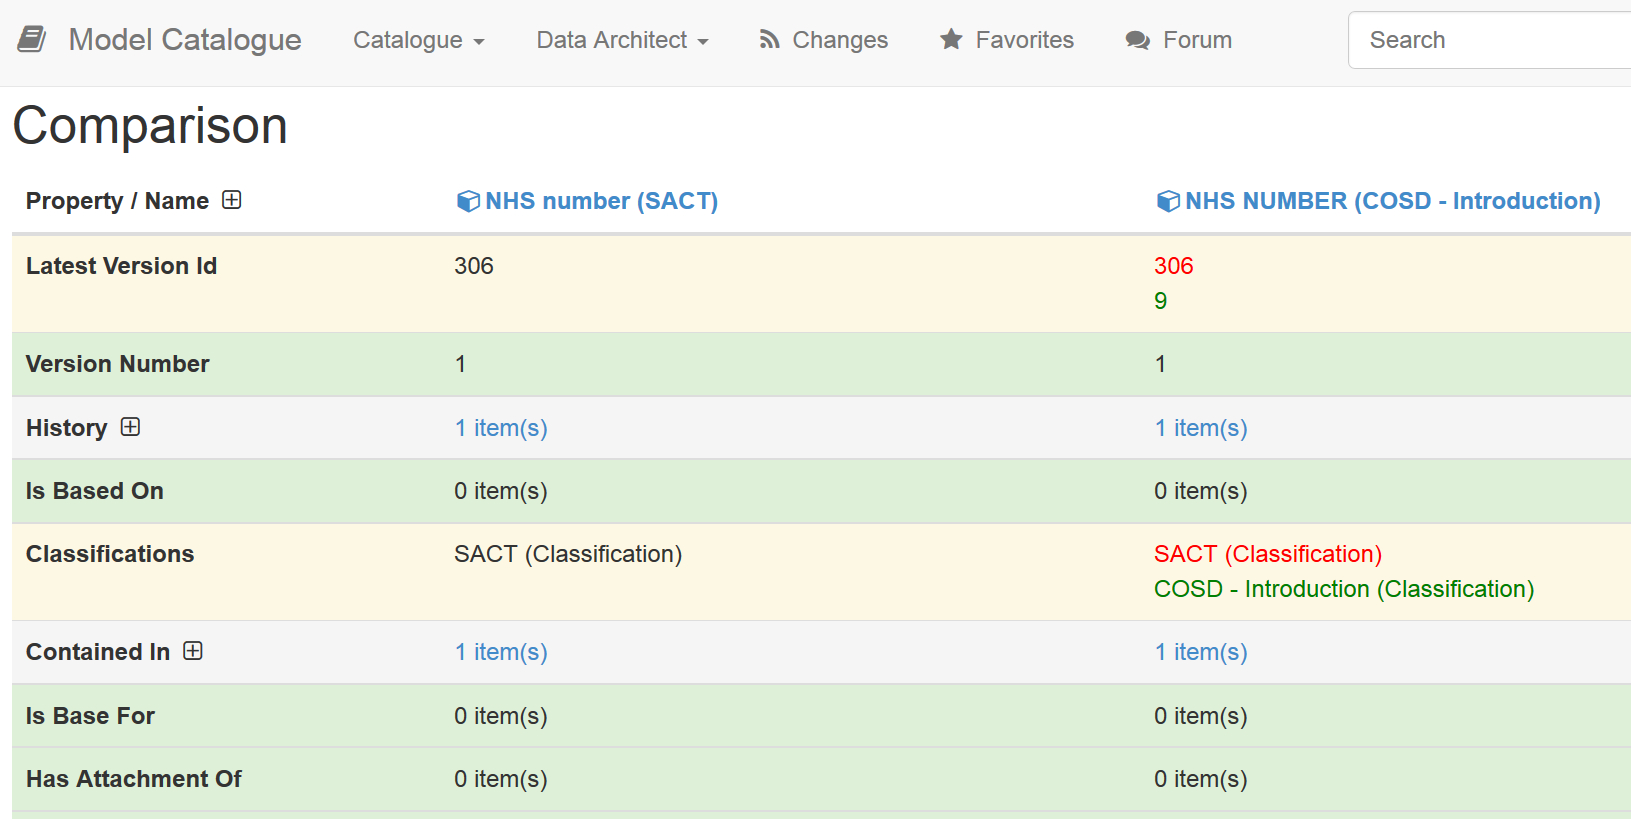
\includegraphics[width= \textwidth,natwidth=610,natheight=642]{ComparisonOfDataClasses.jpg}
	\caption{Screen Shot of DataClass Comparison} 
	\label{fig:dataClassComparison}	
\end{figure*}
\lipsum[3-4]
Whilst that process was being carried out, some of these datasets were added to the Model Catalogue, and the subject matter experts were given visibility of the datasets already stored in the Model Catalogue. At this point the Model Catalogue was already loaded with datasets derived from the NHS Data dictionary such as COSD and from the results of the NHIC work. Use of the toolkit resulted in the users being able to very quickly assemble a new dataset from an existing dataset; they were then able to go through each data element in turn and compare it to an existing data element in another datamodel, a process that is illustrated in Figure~\ref{fig:dataClassComparison}.


 



During the Genomics England project, which is ongoing, the Models Catalogue toolkit has also had a social networking feature added, allowing messaging forums to be automatically generated around a \emph{datamodel} or \emph{dataclass}. This allows users to develop a new draft datamodel, register it as a forum subject and invite other clinicians to comment on it. The result is easier coordination and development of the datasets. 

Two initial tasks in the GE where to assemble datamodels for Cancer and for Rare Diseases. Although these models are still being developed we can report back the facts that to date the new datamodels have been built with a significant amount of re-use as illustrated in the following four tables.

\begin{table}[h]
	\caption{Cancer Data Model : Data-Element Re-use}
	\begin{tabular}{ p{2.8cm} p{1.8cm}  p{1.8cm}   }  % centered columns (3 columns)
		\hline
		DataModel Name &  Elements & \%  \\ 
		\hline
		COSD & 60 & 28.45 \% \\
		NHS Data Dictionary & 12 & 5.7 \% \\
		SACT & 2 & 0.95 \% \\
		New & 137 & 64.9 \% \\
		\hline
		TOTAL & 211
	\end{tabular}
\end{table}

\begin{table}[h]
		\caption{Cancer Data Model : Value Domain / Datatype Re-use}
	\begin{tabular}{p{2.8cm} p{1.8cm}  p{1.8cm}     }  % centered columns (3 columns)
		\hline
		Source & Value Domains& \%  \\ 
		\hline
		NHS Standards & 28 & 20.44\\
		XSD Standard datatypes & 62 & 45.26 \\
		New datatypes & 47 & 34.31 \\
		\hline
		TOTAL & 137
	\end{tabular}
\end{table}

\begin{table}[h]
	\caption{Rare Diseases Data Model : Data-Element Re-use}
	\begin{tabular}{ p{2.8cm} p{1.8cm}  p{1.8cm}   }  % centered columns (3 columns)
		\hline
		DataModel Name &  Elements & \%  \\ 
		\hline
		NHIC & 41 & 10.96 \% \\
		NHS Data Dictionary & 46 & 12.3 \% \\
		New & 287 & 76.74 \% \\
		\hline
		TOTAL & 374
	\end{tabular}
\end{table}

\begin{table}[h]
	\caption{Rare Diseases Data Model : Value Domain / Datatype Re-use}
	\begin{tabular}{ p{2.8cm} p{1.8cm}  p{1.8cm}      }  % centered columns (3 columns)
		\hline
		Source & Value Domains& \%  \\ 
		\hline
		NHS Standards & 81 & 28.22\\
		XSD Standard datatypes & 143 & 49.83 \\
		New datatypes & 63 & 21.95 \\
		\hline
		TOTAL & 137
	\end{tabular}
\end{table}

These figures are a snap-shop of the work in progress, however they are able to illustrate the rate of data element re-use, and of value domain datatype re-use. Both DataModels show an above 20 \% re-use rate for data elements, rising to above 65 \% for the datatypes. The results are significant and indicate that the re-use of both data elements and value types is significant part of the development of disease datamodels, having a model driven toolkit which can assemble a new datamodel and compare it in detail has clearly benefited the clinicians who are now using it.  We admit that the results are not the result of any experiment we have set up to prove the value of the toolkit, but they do strongly support the value of applying model-driven engineering principles in this domain. The time to assemble a new datamodel has been cut from months to weeks as a result of having a single shared source for the datamodel, and having the means to electronically comment on and discuss datamodel development in real time. Unique IRI's identifying each datamodel, dataclass, dataelement and valuedomain mean that searching for entities is fast, comparison between entities is clear and unambiguous, and generating output which conforms to agreed standards becomes straightforward.

 
\section{Lessons actually learned?}

\begin{itemize}
\item metadata registries are not enough - you need models - (we
  should include examples  of how data elements are contextualised -
  Keith slides) - 
\item these models should be linked to the implementation, for
  otherwise it is too expensive to maintain them
\item the models should be readable as data manuals - literate
  modelling - it simply doesn't work to have to click on attributes to
  understand their meaning and derivation 
\item this readability applies to the development interface, this is
  the interface that you want to use (can't do the turn time) - and
  you need to be able to pair program with domain experts
\item you want inheritance within models, and include/import across
  models (start thinking of the models as code, although this is about
  managing information in general - managing declarations - it is
  coincidental that we are generating artefacts from them)
\item you may want different types of model for different generated
  artefacts---depending upon what, exactly, is in the generator code
  as parameters and additional information---it may be the same set of
  data points overall, but you might well have a different refactoring
  in Fowler terms
\item version and store the generation code (!)
\item tag the generated artefacts with a link back to the model
  catalogue (XML schemas in HIC!)
\item you will want more models than you think: for example, consider
  the model of a clinical test; now think about how it is dropped into
  a pathway; you need the pathway model to tell you what the dataset
  means; it has added further context to the data element definitions
  (you could flatten this, but that's bad)
\item automate aspects of model management---versioning and dealing
  with multiple models
  \begin{itemize}
  \item automatically create (and propose) links, including
    classifications
  \item have links for new version of (sequential), refactoring of
    (parallel), derived from (data concepts across models), same as
    (strong assertion)
  \item use links in model maintenance - note that the definition that
    this was derived from has changed
  \item have publication cycle---a published model is for life
  \end{itemize}
\item general lesson: if you want to manage data semantics, you need a
  compositional approach---none of this central coordination of a
  single data dictionary, none of this single hierarchy of data
  elements, none of this element by element description (all the
  context in the text of the element definition?  doesn't work!)
\item general lesson: if you are going to manage data at scale, you
  need data model driven approach
\item general lesson: if you have a model driven approach (data model
  or otherwise) then your management of models has all the same
  challenges as management of source code (you need an IDE) - really,
  if you are using models as programs, then you need to support them
  as programs
\end{itemize}